\section{Balanceamento}

Consideremos um rotor biapoiado por mancais em ambas extremidades que gira em relação ao seu eixo Z.

\begin{center}
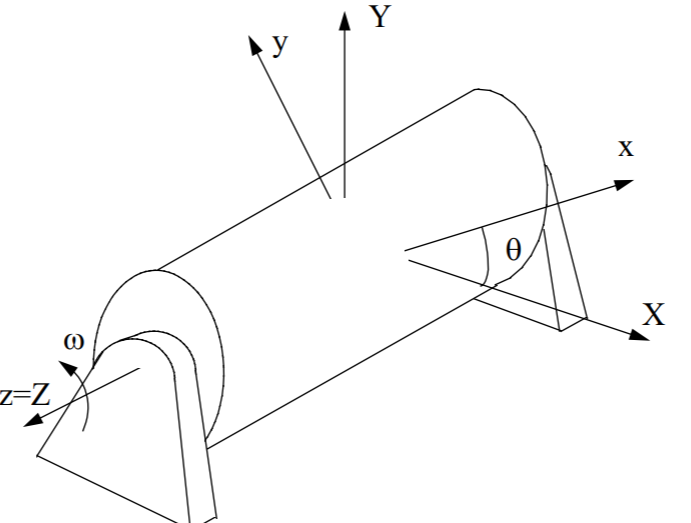
\includegraphics[width=8cm]{C:/Users/patri/Downloads/Poli/lateco/mecanica/figuras/rotor.png}
\end{center}

\subsection{Rotor desbalanceado}

Temos que as equações que configuram o movimento de um rotor desbalanceado são

$$
\begin{cases}

(z_AA_y + z_BB_y) = -(J_{XZ}\ddot{\theta} - J_{YZ}\dot{\theta^2})\\
(z_AA_x + z_BB_x) = -(J_{YZ}\ddot{\theta} - J_{XZ}\dot{\theta^2}) - X_GPsen(\alpha) \\ 
J_Z\ddot{\theta} = H - x_gPcos(\alpha)cos(\theta)

\end{cases}$$

e

$$
\begin{cases}
A_x + B_x = Pcos(\alpha)sen(\theta) - m\dot{\theta}^2x_G \\
A_y + B_y = Pcos(\alpha)cos(\theta) + m\dot{\theta}^2x_g \\
A_z + B_z = Psen(\alpha)

\end{cases}
$$

Onde $\alpha$ é o angulo formado pelo eixo normal ao rotor e a horizontal.
É possível verificar que dados condições de contorno $(\theta, \dot{\theta})$ pode-se integrar as equações acima para encontrar as reações dinâmicas $(A_x, A_y, B_x, B_y)$

\subsection{Rotor balanceado}

\begin{namedtheorem}[Balanceamento Estático]
Centro de massa do sistema deve estar no eixo de rotação do sistema. Com isso, retira-se o momento gerado pelo peso das equações acima.
\end{namedtheorem}

\begin{namedtheorem}[Balanceamento Dinâmico]
Matriz diagonal deve ser nula, portanto deve-se zerar os momentos de inercia, o que irá zerar os termos que multiplicam os momentos de inercia nas equações acima.
\end{namedtheorem}

As equações resultantes são:

$$
\begin{cases}

(z_AA_y + z_BB_y) = 0\\
(z_AA_x + z_BB_x) = 0\\ 
J_Z\ddot{\theta} = H

\end{cases}$$

e

$$
\begin{cases}
A_x + B_x = Pcos(\alpha)sen(\theta)\\
A_y + B_y = Pcos(\alpha)cos(\theta)\\
A_z + B_z = Psen(\alpha)

\end{cases}
$$

\begin{namedtheorem}[Condições de balanceamento]
Portanto as condições de balanceamento são:

\begin{itemize}
	\item $X_g = 0$
	\item $Y_g = 0$
	\item $J_{xz} = 0$
	\item $J_{yz} = 0$
\end{itemize}
\end{namedtheorem}











